% Options for packages loaded elsewhere
\PassOptionsToPackage{unicode}{hyperref}
\PassOptionsToPackage{hyphens}{url}
%
\documentclass[
  man, donotrepeattitle,floatsintext]{apa7}
\usepackage{amsmath,amssymb}
\usepackage{lmodern}
\usepackage{iftex}
\ifPDFTeX
  \usepackage[T1]{fontenc}
  \usepackage[utf8]{inputenc}
  \usepackage{textcomp} % provide euro and other symbols
\else % if luatex or xetex
  \usepackage{unicode-math}
  \defaultfontfeatures{Scale=MatchLowercase}
  \defaultfontfeatures[\rmfamily]{Ligatures=TeX,Scale=1}
\fi
% Use upquote if available, for straight quotes in verbatim environments
\IfFileExists{upquote.sty}{\usepackage{upquote}}{}
\IfFileExists{microtype.sty}{% use microtype if available
  \usepackage[]{microtype}
  \UseMicrotypeSet[protrusion]{basicmath} % disable protrusion for tt fonts
}{}
\makeatletter
\@ifundefined{KOMAClassName}{% if non-KOMA class
  \IfFileExists{parskip.sty}{%
    \usepackage{parskip}
  }{% else
    \setlength{\parindent}{0pt}
    \setlength{\parskip}{6pt plus 2pt minus 1pt}}
}{% if KOMA class
  \KOMAoptions{parskip=half}}
\makeatother
\usepackage{xcolor}
\usepackage{graphicx}
\makeatletter
\def\maxwidth{\ifdim\Gin@nat@width>\linewidth\linewidth\else\Gin@nat@width\fi}
\def\maxheight{\ifdim\Gin@nat@height>\textheight\textheight\else\Gin@nat@height\fi}
\makeatother
% Scale images if necessary, so that they will not overflow the page
% margins by default, and it is still possible to overwrite the defaults
% using explicit options in \includegraphics[width, height, ...]{}
\setkeys{Gin}{width=\maxwidth,height=\maxheight,keepaspectratio}
% Set default figure placement to htbp
\makeatletter
\def\fps@figure{htbp}
\makeatother
\setlength{\emergencystretch}{3em} % prevent overfull lines
\providecommand{\tightlist}{%
  \setlength{\itemsep}{0pt}\setlength{\parskip}{0pt}}
\setcounter{secnumdepth}{-\maxdimen} % remove section numbering
% Make \paragraph and \subparagraph free-standing
\ifx\paragraph\undefined\else
  \let\oldparagraph\paragraph
  \renewcommand{\paragraph}[1]{\oldparagraph{#1}\mbox{}}
\fi
\ifx\subparagraph\undefined\else
  \let\oldsubparagraph\subparagraph
  \renewcommand{\subparagraph}[1]{\oldsubparagraph{#1}\mbox{}}
\fi
\ifLuaTeX
\usepackage[bidi=basic]{babel}
\else
\usepackage[bidi=default]{babel}
\fi
\babelprovide[main,import]{english}
% get rid of language-specific shorthands (see #6817):
\let\LanguageShortHands\languageshorthands
\def\languageshorthands#1{}
% Manuscript styling
\usepackage{upgreek}
\captionsetup{font=singlespacing,justification=justified}

% Table formatting
\usepackage{longtable}
\usepackage{lscape}
% \usepackage[counterclockwise]{rotating}   % Landscape page setup for large tables
\usepackage{multirow}		% Table styling
\usepackage{tabularx}		% Control Column width
\usepackage[flushleft]{threeparttable}	% Allows for three part tables with a specified notes section
\usepackage{threeparttablex}            % Lets threeparttable work with longtable

% Create new environments so endfloat can handle them
% \newenvironment{ltable}
%   {\begin{landscape}\centering\begin{threeparttable}}
%   {\end{threeparttable}\end{landscape}}
\newenvironment{lltable}{\begin{landscape}\centering\begin{ThreePartTable}}{\end{ThreePartTable}\end{landscape}}

% Enables adjusting longtable caption width to table width
% Solution found at http://golatex.de/longtable-mit-caption-so-breit-wie-die-tabelle-t15767.html
\makeatletter
\newcommand\LastLTentrywidth{1em}
\newlength\longtablewidth
\setlength{\longtablewidth}{1in}
\newcommand{\getlongtablewidth}{\begingroup \ifcsname LT@\roman{LT@tables}\endcsname \global\longtablewidth=0pt \renewcommand{\LT@entry}[2]{\global\advance\longtablewidth by ##2\relax\gdef\LastLTentrywidth{##2}}\@nameuse{LT@\roman{LT@tables}} \fi \endgroup}

% \setlength{\parindent}{0.5in}
% \setlength{\parskip}{0pt plus 0pt minus 0pt}

% Overwrite redefinition of paragraph and subparagraph by the default LaTeX template
% See https://github.com/crsh/papaja/issues/292
\makeatletter
\renewcommand{\paragraph}{\@startsection{paragraph}{4}{\parindent}%
  {0\baselineskip \@plus 0.2ex \@minus 0.2ex}%
  {-1em}%
  {\normalfont\normalsize\bfseries\itshape\typesectitle}}

\renewcommand{\subparagraph}[1]{\@startsection{subparagraph}{5}{1em}%
  {0\baselineskip \@plus 0.2ex \@minus 0.2ex}%
  {-\z@\relax}%
  {\normalfont\normalsize\itshape\hspace{\parindent}{#1}\textit{\addperi}}{\relax}}
\makeatother

% \usepackage{etoolbox}
\makeatletter
\patchcmd{\HyOrg@maketitle}
  {\section{\normalfont\normalsize\abstractname}}
  {\section*{\normalfont\normalsize\abstractname}}
  {}{\typeout{Failed to patch abstract.}}
\patchcmd{\HyOrg@maketitle}
  {\section{\protect\normalfont{\@title}}}
  {\section*{\protect\normalfont{\@title}}}
  {}{\typeout{Failed to patch title.}}
\makeatother

\usepackage{xpatch}
\makeatletter
\xapptocmd\appendix
  {\xapptocmd\section
    {\addcontentsline{toc}{section}{\appendixname\ifoneappendix\else~\theappendix\fi\\: #1}}
    {}{\InnerPatchFailed}%
  }
{}{\PatchFailed}
\usepackage{csquotes}
\usepackage{newtxtext,newtxmath}
\usepackage{pdflscape}
\AtBeginDocument{\let\maketitle\relax}
\usepackage{longtable}
\usepackage{graphicx}
\usepackage{graphbox}
\usepackage{tabularray}
\UseTblrLibrary{booktabs}
\raggedbottom
\pagenumbering{gobble}
\ifLuaTeX
  \usepackage{selnolig}  % disable illegal ligatures
\fi
\IfFileExists{bookmark.sty}{\usepackage{bookmark}}{\usepackage{hyperref}}
\IfFileExists{xurl.sty}{\usepackage{xurl}}{} % add URL line breaks if available
\urlstyle{same} % disable monospaced font for URLs
\hypersetup{
  pdftitle={The combination of reporting bias and underpowered study designs has substantially exaggerated the motor learning benefits of self-controlled practice and enhanced expectancies: A meta-analysis},
  pdflang={en-EN},
  hidelinks,
  pdfcreator={LaTeX via pandoc}}

\title{The combination of reporting bias and underpowered study designs has substantially exaggerated the motor learning benefits of self-controlled practice and enhanced expectancies: A meta-analysis}
\author{\phantom{0}}
\date{}


\shorttitle{Motivation pillar of OPTIMAL theory}

\affiliation{\phantom{0}}

\begin{document}
\maketitle

\renewcommand{\arraystretch}{1.7}
\DefTblrTemplate{caption-tag}{default}{Table\hspace{0.25em}\thetable}
\DefTblrTemplate{caption-sep}{default}{.\enskip}
\DefTblrTemplate{caption-text}{default}{\InsertTblrText{caption}}
\DefTblrTemplate{contfoot-text}{default}{(\emph{Continued})}
\DefTblrTemplate{middlehead,lasthead}{default}{\textbf{Table 1.} Continued}
\SetTblrStyle{caption-tag,caption-sep}{\bfseries}
\small
\begin{longtblr}[
  caption = {The selection and regression models used in our robust Bayesian meta-analysis approach.},
  label = {tab:table1},
]{colspec = {p{4.8cm}p{5cm}p{4.8cm}}}
\toprule
  \textbf{Type of selection} &
  \textbf{Visualization} &
  \textbf{Example scenario} \\ 
\midrule
  \textbf{\underline{Selection models}} &
  &
  \textbf{\underline{Direction not important}} \\
Significant results are more likely to be reported in either direction (two-tailed)  &
  \raisebox{-0.9\height}{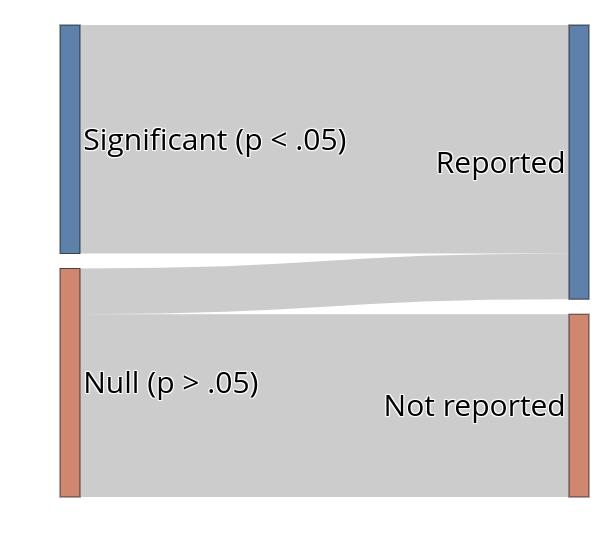
\includegraphics[width=4.75cm]{../../figs/model1.png}} &
  Researcher conducts test and observes a null result. They decide the experiment did not work and move on. Significant results get reported. \\
Significant results are most likely to be reported, but `non-significant trends' are more likely to be reported than other null results in either direction (two-tailed). &
  \raisebox{-0.9\height}{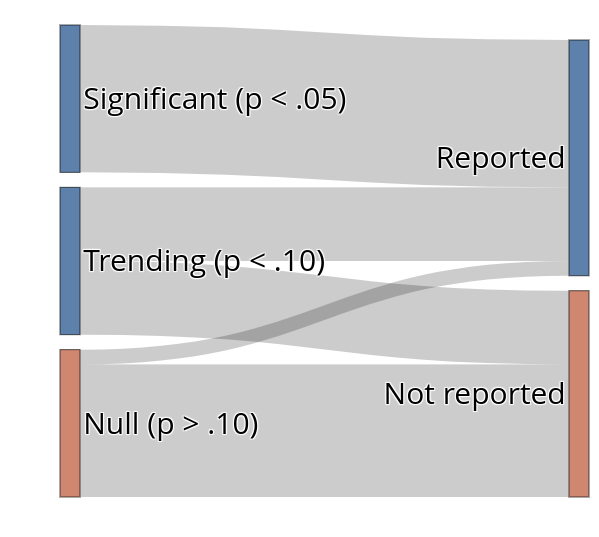
\includegraphics[width=4.75cm]{../../figs/model2.png}} &
  Authors report significant results and `non-significant trends'. The latter may be interpreted as fair evidence the manipulation worked. Some reviewers take issue with trends, so only some make it through and get reported. Null results unlikely to be written up. \\
  &
  &
  \textbf{\underline{Direction important}} \\
Significant results and non-significant trends are more likely to be reported in the predicted direction. &
  \raisebox{-0.9\height}{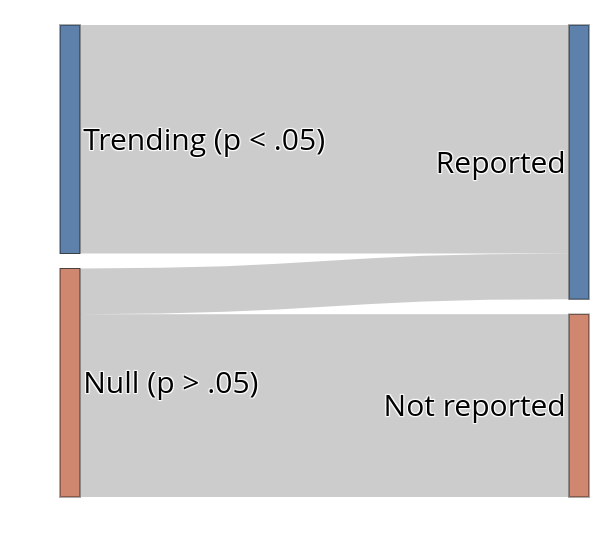
\includegraphics[width=4.75cm]{../../figs/model3.png}} &
  Researcher is confident in the hypothesis being tested in an experiment and doubts the validity of null or opposing findings. Reports results they are confident in. \\
Significant results in the predicted direction are more likely to be reported than trends, which are more likely to be reported than other null results and significant results in the opposite (i.e., `wrong') direction. &
  \raisebox{-0.9\height}{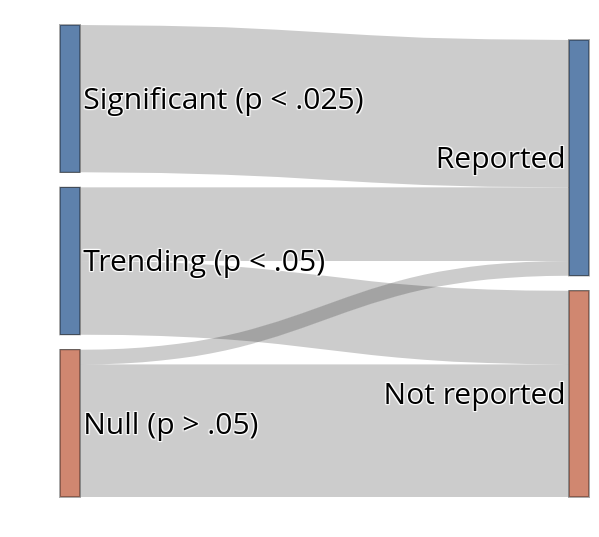
\includegraphics[width=4.75cm]{../../figs/model4.png}} &
  A preference for reporting findings with a compelling narrative results in preferring significant results and occasionally trends. Null or conflicting results less likely to add to the narrative. \\
Significant results and trends in the predicted (i.e., `correct') direction are more likely to be reported than null findings in the predicted (i.e., `correct') direction, which are more likely to be reported than results in the opposite (i.e., `wrong') direction. &
  \raisebox{-0.9\height}{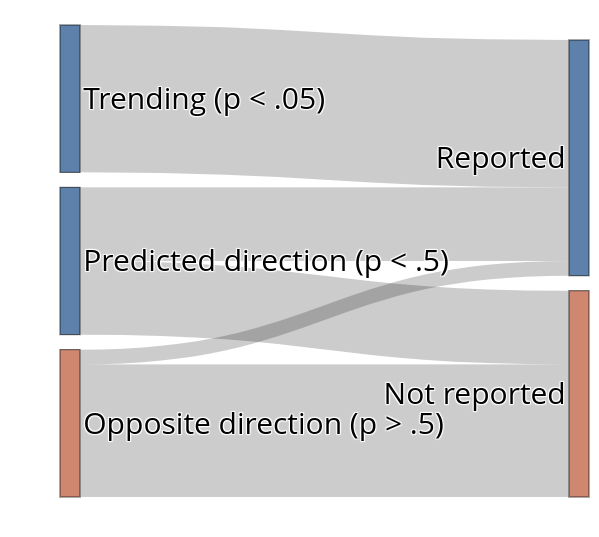
\includegraphics[width=4.75cm]{../../figs/model5.png}} &
  A student observes results in the opposite direction of what was expected. Supervisor thinks something may have went wrong so results not published. Other students publish results consistent with predictions. \\
Full selection model. Significant results most likely, then trends, then null results in the predicted (i.e., `correct') direction. The least likely to be reported are results in the opposite (i.e., `wrong') direction. &
  \raisebox{-0.9\height}{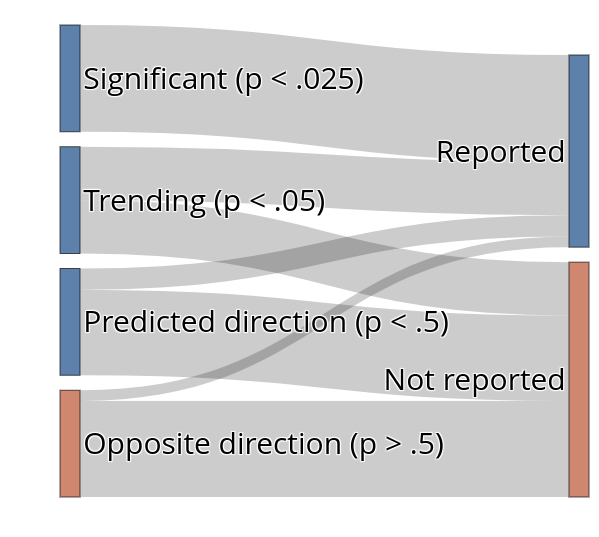
\includegraphics[width=4.75cm]{../../figs/model6.png}} &
  An editor prefers to publish interesting results. Prediction successes are interesting. Some trends are interesting if they are believable. Results in the opposite direction are interesting, but only if replicated. \vspace{1em} \\
  \textbf{\underline{Regression models}} &
  &
  \\
Conditioning on smaller \emph{p}-values in the predicted direction creates a relationship between effect sizes and standard errors. Called `small study effects' because all else being equal smaller studies need larger effects to achieve significant results. &
  \raisebox{-0.9\height}{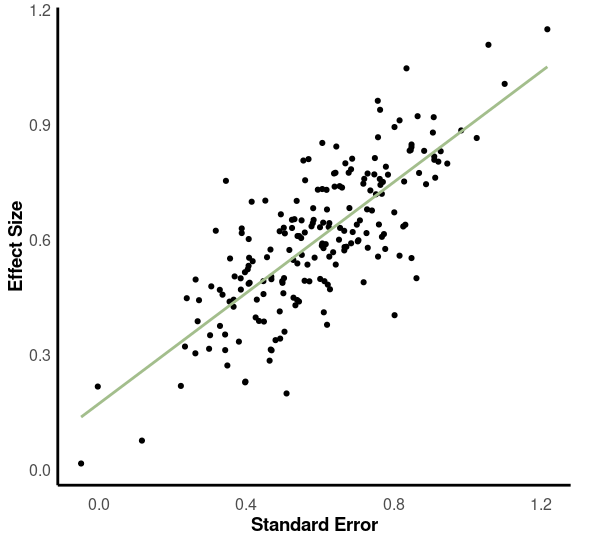
\includegraphics[width=4.75cm]{../../figs/model7.png}} &
  This models the dependency caused by selective reporting, not the underlying mechanism itself. Dependency can be caused by a third variable, such as intensity of the interventions used in smaller compared to larger studies. \\
Quadratic relationship between effect and standard errors. Large studies likely to be reported independent of results, while smaller studies need increasingly large effects in the predicted (i.e., `correct') direction to avoid censorship. &
  \raisebox{-0.9\height}{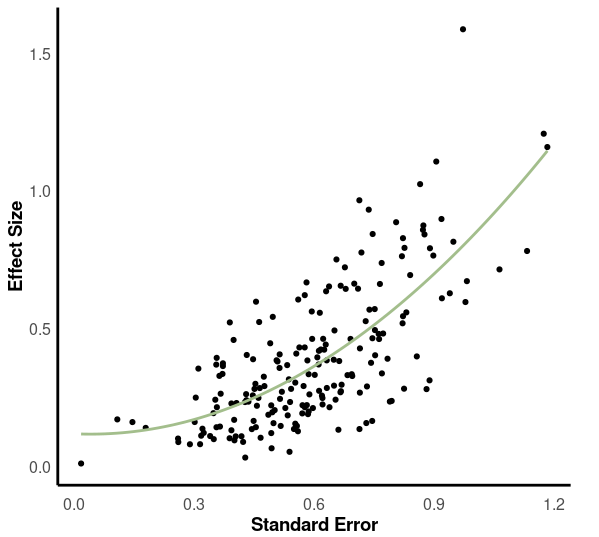
\includegraphics[width=4.75cm]{../../figs/model8.png}} &
  Researchers invest in conducting a large study and are motivated to publish regardless of the results. They persevere if null results are rejected. Small studies are abandoned unless the results are impressive. \\
\bottomrule
\end{longtblr}


\end{document}
